\setcounter{ex}{0} %Ba Đồn-Quảng Bình
\subsection{Trắc nghiệm (2 điểm)}
\Opensolutionfile{ans}[ans/ans7]


%%Câu 1:
\begin{ex}
Tìm giá trị của tham số $m$ để hệ phương trình
$\begin{cases}
2x-3y=5\\
(m+1)x-6y=m+3
\end{cases}$
vô nghiệm.
\vspace{0.35cm}
\choice
{\True $m=3$}
{$m=-1$}
{$m=0$}
{$m=5$}
\end{ex}

%%Câu 2:
\begin{ex}
Tổng các nghiệm của phương trình $\dfrac{1}{x+3}+\dfrac{2}{x-3}=\dfrac{x^2+3}{x^2-9}$ bằng
\vspace{0.35cm}
\choice
{$3$}
{$2$}
{$4$}
{\True $0$}
\end{ex}

%%Câu 3:
\begin{ex}
Cho hai đường tròn đồng tâm có bán kính lần lượt là $9\,\text{cm}$ và $6\,\text{cm}$. Phần hình vành khuyên nằm trong một góc ở tâm $120^\circ$ có diện tích bằng
\choice
{$20\pi\,\text{cm}^2$}
{$45\pi\,\text{cm}^2$}
{$30\pi\,\text{cm}^2$}
{\True $15\pi\,\text{cm}^2$}
\end{ex}

%%Câu 4:
\begin{ex}
Tính tổng các giá trị nguyên $x$ thỏa mãn cả hai bất phương trình
$\begin{cases}
2x+1<4x+5\\
3x-1<\dfrac{x}{2}+4
\end{cases}$.
\choice
{$4$}
{$2$}
{\True $0$}
{$1$}
\end{ex}

%%Câu 5:
\begin{ex}
Cho biểu thức
$A=\sqrt{(2x-3)^2}-\sqrt{(x+1)^2}$.
Rút gọn biểu thức $A$ với $-1\le x<\dfrac{3}{2}$, ta được
\choice
{$4-x$}
{\True $2-3x$}
{$2+x$}
{$3x-2$}
\end{ex}

%%Câu 6:
\begin{ex}
Cho tam giác $ABC$ vuông tại $A$, đường cao $AH$ và $AB=30$, $BH=18$. Chu vi tam giác $ABC$ là
\choice
{\True $120$}
{$130$}
{$125$}
{$110$}
\end{ex}

%%Câu 7:
\begin{ex}
Cho hai đường tròn $(O;9\,\text{cm})$ và $(O';4\,\text{cm})$ có $OO'=5\,\text{cm}$. Khẳng định nào sau đây đúng về vị trí tương đối của hai đường tròn?
\choice
{\True Hai đường tròn tiếp xúc trong}
{Hai đường tròn tiếp xúc ngoài}
{Hai đường tròn cắt nhau tại hai điểm}
{Hai đường tròn ở ngoài nhau}
\end{ex}

%%Câu 8:
\begin{ex}
Phương trình $5x(-10x-2)=90x+18$ tương đung với phương trình nào sau đây?
\choice
{$(-10x-2)(5x+10)=0$}
{$(1-10x)(5x+9)=0$}
{\True $(-10x-2)(5x+9)=0$}
{$(2-10x)(5x+9)=0$}
\end{ex}

%%Câu 9:
\begin{ex}
Cho đường tròn $(O;12\,\text{cm})$. Một cung nhỏ của đường tròn có số đo $135^\circ$. Độ dài của cung nhỏ đó bằng
\choice
{$6\pi\,\text{cm}$}
{$12\pi\,\text{cm}$}
{$18\pi\,\text{cm}$}
{\True $9\pi\,\text{cm}$}
\end{ex}

%%Câu 10:
\begin{ex}
Cho đường tròn $(O;5\,\text{cm})$ và điểm $P$ nằm ngoài đường tròn sao cho $OP=13\,\text{cm}$. Từ $P$ kẻ tiếp tuyến $PA$ với đường tròn $(O)$ ($A$ là tiếp điểm). Độ dài đoạn thẳng $PA$ bằng
\choice
{$\sqrt{194}\,\text{cm}$}
{\True $12\,\text{cm}$}
{$8\,\text{cm}$}
{$18\,\text{cm}$}
\end{ex}


\Closesolutionfile{ans}
\Opensolutionfile{ansbook}[ans/ansbook7]
\setcounter{bt}{0}
\subsection{Tự luận (8 điểm)}

%Bài 1:
\begin{bt}[1,5 điểm]
Giải các phương trình, bất phương trình và hệ phương trình sau:
\begin{listEX}[3]
\item $(3x-2)^2-(x+4)^2=0$
\item $\dfrac{3x-2}{4}-\dfrac{x+5}{3}<\dfrac{5x+1}{6}$
\item $\begin{cases}
\dfrac{2x-y}{3}+\dfrac{x+2y}{2}=\dfrac{5}{3}\\
3(x-1)-2(y+2)=1
\end{cases}$
\end{listEX}
\loigiai{
\begin{enumerate}
\item Ta có
\begin{align*}
(3x-2)^2-(x+4)^2&=0\\
\big[(3x-2)-(x+4)\big]\big[(3x-2)+(x+4)\big]&=0\\
(2x-6)(4x+2)&=0.
\end{align*}
Do đó $x=3$ hoặc $x=-\dfrac{1}{2}$.

\item Nhân cả hai vế với $12>0$, ta được
\begin{align*}
3(3x-2)-4(x+5)&<2(5x+1)\\
5x-26&<10x+2\\
-28&<5x\\
x&>-\dfrac{28}{5}.
\end{align*}
Vậy bất phương trình có nghiệm $x>-\dfrac{28}{5}$.

\item Dùng phương pháp cộng đại số, ta có
\begin{align*}
&\begin{cases}
\dfrac{2x-y}{3}+\dfrac{x+2y}{2}=\dfrac{5}{3},\\
3(x-1)-2(y+2)=1
\end{cases}\\[0.7em]
\Leftrightarrow\quad
&\begin{cases}
7x+4y=10,\\
3x-2y=8
\end{cases}\\[0.7em]
\Leftrightarrow\quad
&\begin{cases}
7x+4y=10,\\
6x-4y=16
\end{cases}\\[0.7em]
\Leftrightarrow\quad
&\begin{cases}
13x=26,\\
3x-2y=8
\end{cases}\\[0.7em]
\Leftrightarrow\quad
&\begin{cases}
x=2,\\
y=-1.
\end{cases}
\end{align*}
Vậy hệ phương trình có nghiệm $(x;y)=(2;-1)$.
\end{enumerate}
}
\end{bt}


%Bài 2

\begin{bt}[1 điểm]
Rút gọn các biểu thức sau:
\begin{listEX}[2]
\item $\sqrt{23+8\sqrt{7}}+\sqrt{23-8\sqrt{7}}-\sqrt{14-4\sqrt{10}}$
\item $\dfrac{\sqrt{80}-\sqrt{5}}{\sqrt{5}-\sqrt{3}}+\dfrac{3\sqrt{3}}{\sqrt{5}+\sqrt{3}}$
\end{listEX}
\loigiai{
\begin{enumerate}
\setlength{\itemsep}{1em}

\item Ta có
\begin{align*}
23+8\sqrt{7}
&=16+2\cdot4\sqrt{7}+7\\
&=\left(4+\sqrt{7}\right)^2,\\
23-8\sqrt{7}
&=16-2\cdot4\sqrt{7}+7\\
&=\left(4-\sqrt{7}\right)^2,\\
14-4\sqrt{10}
&=10-2\cdot\sqrt{10}\cdot2+4\\
&=\left(\sqrt{10}-2\right)^2.
\end{align*}
Vì $4-\sqrt{7}>0$ và $\sqrt{10}-2>0$ nên
\begin{align*}
\sqrt{23+8\sqrt{7}}+\sqrt{23-8\sqrt{7}}
-\sqrt{14-4\sqrt{10}}\\
&=4+\sqrt{7}+4-\sqrt{7}-\left(\sqrt{10}-2\right)\\
&=10-\sqrt{10}.
\end{align*}
Vậy biểu thức đã cho rút gọn thành $10-\sqrt{10}$.

\item Ta có $\sqrt{80}=4\sqrt{5}$, do đó
\begin{align*}
\dfrac{\sqrt{80}-\sqrt{5}}{\sqrt{5}-\sqrt{3}}
+\dfrac{3\sqrt{3}}{\sqrt{5}+\sqrt{3}}\\
&=\dfrac{3\sqrt{5}}{\sqrt{5}-\sqrt{3}}
+\dfrac{3\sqrt{3}}{\sqrt{5}+\sqrt{3}}\\
&=\dfrac{3\sqrt{5}\left(\sqrt{5}+\sqrt{3}\right)}{5-3}
+\dfrac{3\sqrt{3}\left(\sqrt{5}-\sqrt{3}\right)}{5-3}\\
&=\dfrac{15+3\sqrt{15}+3\sqrt{15}-9}{2}\\
&=3+3\sqrt{15}.
\end{align*}
Vậy biểu thức đã cho rút gọn thành $3+3\sqrt{15}$.
\end{enumerate}
}
\end{bt}

%Bài 3
\begin{bt}[1,0 điểm]
Cô Hà mua dụng cụ học tập tại một cửa hàng. Lần thứ nhất, cô mua $5$ cây bút và $3$ quyển vở hết $70\,000$ đồng. Lần thứ hai, cô mua $2$ cây bút và $4$ quyển vở hết $56\,000$ đồng. Biết các cây bút cùng giá và các quyển vở cùng giá. Tính giá tiền của một cây bút và một quyển vở.
\loigiai{
Gọi $x$ (nghìn đồng) là giá một cây bút và $y$ (nghìn đồng) là giá một quyển vở, với $x>0$, $y>0$.

Lần mua thứ nhất cho ta
\[
5x+3y=70. \tag{1}
\]
Lần mua thứ hai cho ta
\[
2x+4y=56. \tag{2}
\]
Chia hai vế của $(2)$ cho $2$:
\[
x+2y=28 \Rightarrow x=28-2y. \tag{3}
\]
Thế $(3)$ vào $(1)$:
\begin{align*}
5(28-2y)+3y&=70\\
140-10y+3y&=70\\
140-7y&=70\\
-7y&=-70\\
y&=10.
\end{align*}
Thay $y=10$ vào $(3)$:
\[
x=28-2\cdot 10=8.
\]
Cặp $(x;y)=(8;10)$ thỏa $x>0$, $y>0$.

\emph{Kiểm tra.}
\(5\cdot 8+3\cdot 10=70\) và \(2\cdot 8+4\cdot 10=56\), đúng với giả thiết.

Vậy một cây bút giá $8\,000$ đồng và một quyển vở giá $10\,000$ đồng.
}
\end{bt}

%Bài 4

\begin{bt}[1,0 điểm]
	Tính chiều cao $CD$ của một ngọn núi, biết tại hai điểm $A$ và $B$ cách nhau $1$ km trên mặt đất, người ta nhìn thấy đỉnh núi $D$ với góc nâng lần lượt là $30^\circ$ và $45^\circ$ (làm tròn đến hai chữ số thập phân sau dấu phẩy).
	\begin{center}
		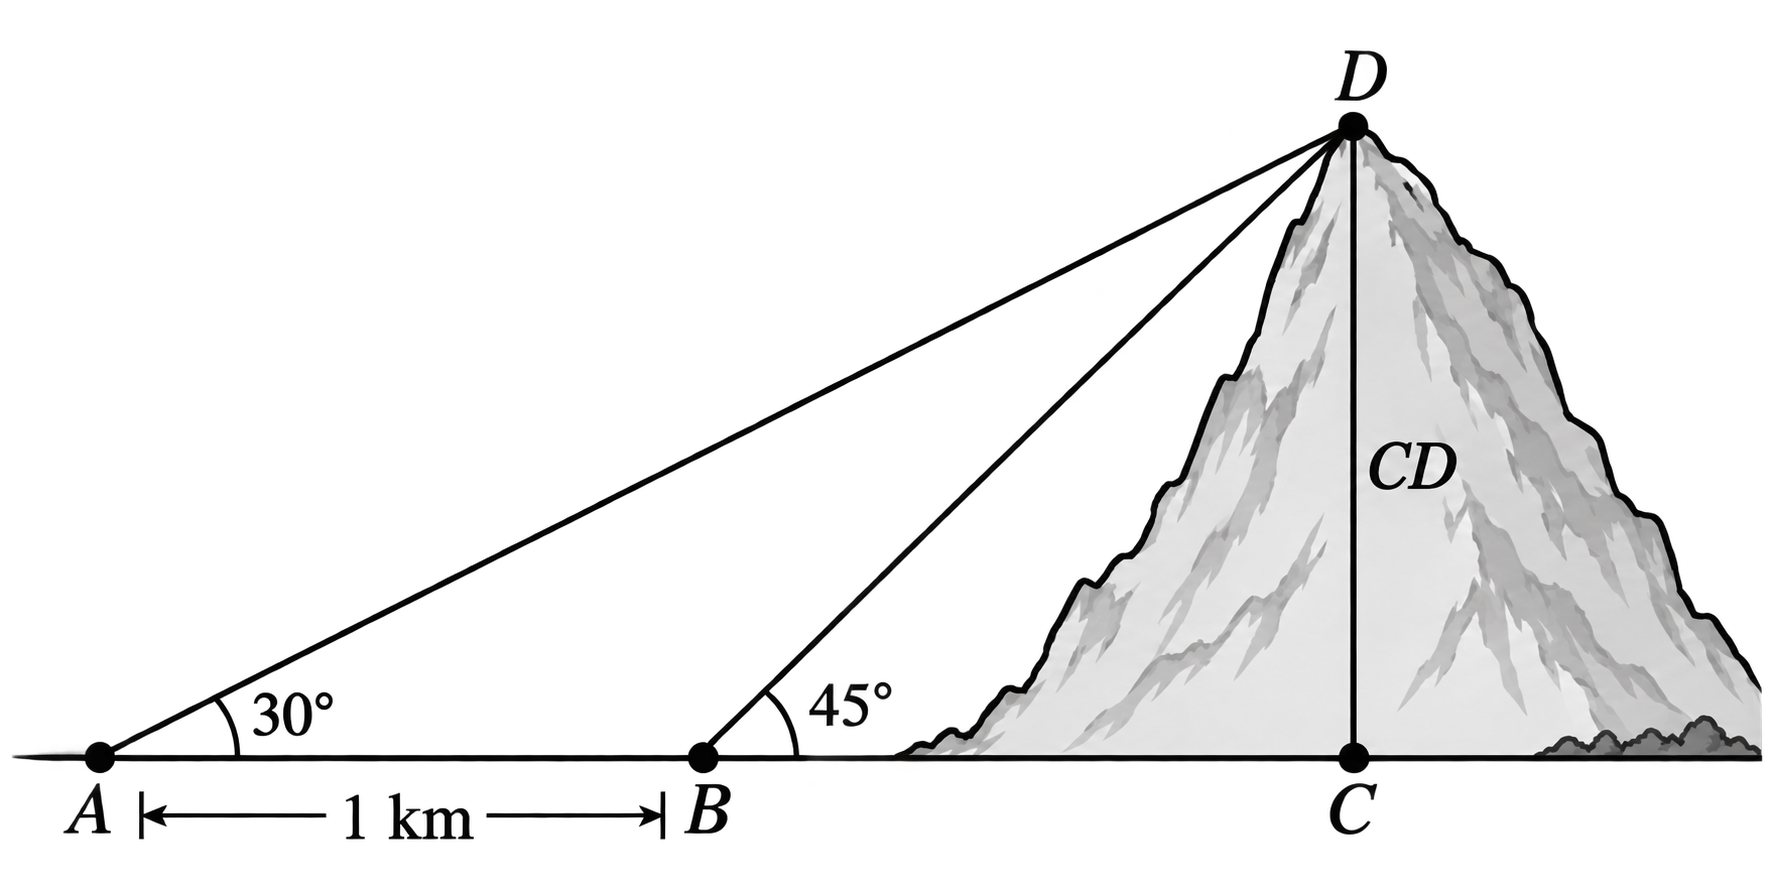
\includegraphics[width=0.45\textwidth]{hinh/De7-cau4.png}
	\end{center}
	
	\loigiai{
	Đổi $1$ km $=1000$ m.
	
	Xét tam giác $DCB$ vuông tại $C$, ta có:
	\[
	\tan\widehat{DBC}=\dfrac{DC}{BC}
	\Rightarrow BC=\dfrac{DC}{\tan45^\circ}.
	\]
	
	Xét tam giác $DCA$ vuông tại $C$, ta có:
	\[
	\tan\widehat{DAC}=\dfrac{DC}{AC}
	\Rightarrow AC=\dfrac{DC}{\tan30^\circ}.
	\]
	
	Ta có:
	\[
	AC-BC=AB
	\Rightarrow
	\dfrac{DC}{\tan30^\circ}
	-\dfrac{DC}{\tan45^\circ}
	=1000.
	\]
	
	Suy ra:
	\[
	DC\left(
	\dfrac{1}{\tan30^\circ}
	-\dfrac{1}{\tan45^\circ}
	\right)=1000.
	\]
	
	Vậy chiều cao của ngọn núi là
	\[
	DC=1000:
	\left(
	\dfrac{1}{\tan30^\circ}
	-\dfrac{1}{\tan45^\circ}
	\right)
	\approx 1366{,}03\text{ (m)}.
	\]
	}
\end{bt}
	

%Câu 5
\begin{bt}[1,0 điểm]
\immini[thm]
{Một tấm gỗ hình tròn bán kính $16$ cm được gắn chính giữa một gương tròn bán kính $10$ cm. Phần gỗ còn nhìn thấy là một hình vành khuyên (hình vẽ). Lấy $\pi=3{,}14$.
\begin{enumerate}
\item Tính diện tích phần gỗ còn nhìn thấy (làm tròn kết quả đến hàng phần mười centimét vuông).
\item Người ta dán một đường kim tuyến quanh mép ngoài của tấm gỗ. Tính độ dài đường kim tuyến đó (làm tròn kết quả đến hàng phần mười centimét).
\end{enumerate}
}
{
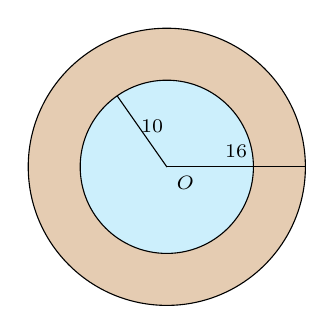
\begin{tikzpicture}[scale=0.11, font=\scriptsize, line join=round]
	\fill[brown!40] (0,0) circle (16);
	\fill[cyan!20] (0,0) circle (10);
	\draw (0,0) circle (16);
	\draw (0,0) circle (10);
	\draw (0,0)--(16,0);
	\node[above] at (8,0) {$16$};
	\draw (0,0)--(125:10);
	\node[above right] at (145:5) {$10$};
	\fill (0,0) circle (2pt) node[below right] {$O$};
\end{tikzpicture}
}
\loigiai{
\begin{enumerate}
\item Phần gỗ còn nhìn thấy là hình vành khuyên có bán kính ngoài $R=16$ cm và bán kính trong $r=10$ cm. Diện tích phần này là
\begin{align*}
S&=\pi R^2-\pi r^2\\
&=\pi\left(16^2-10^2\right)\\
&=3{,}14(256-100)\\
&=3{,}14\cdot 156\\
&=489{,}84\ \text{(cm}^2\text{)}.
\end{align*}
Làm tròn đến hàng phần mười: $S\approx 489{,}8$ cm$^2$.

Vậy diện tích phần gỗ còn nhìn thấy khoảng $489{,}8$ cm$^2$.

\item Đường kim tuyến là chu vi đường tròn mép ngoài, bán kính $16$ cm:
\begin{align*}
C&=2\pi R\\
&=2\cdot 3{,}14\cdot 16\\
&=100{,}48\ \text{(cm)}.
\end{align*}
Làm tròn đến hàng phần mười: $C\approx 100{,}5$ cm.

Vậy độ dài đường kim tuyến khoảng $100{,}5$ cm.
\end{enumerate}
}
\end{bt}

%Bài 6
\begin{bt}[2,5 điểm]
Cho nửa đường tròn $(O)$, đường kính $AB=2R$. Trên nửa đường tròn lấy điểm $C$ bất kì ($C$ khác $A$ và $B$). Tiếp tuyến tại $C$ và tiếp tuyến tại $A$ cắt nhau tại $M$.
\begin{enumerate}
\item Chứng minh bốn điểm $O$, $M$, $A$, $C$ cùng thuộc một đường tròn.
\item $AC$ cắt $OM$ tại $H$. Chứng minh $AC\perp OM$ và $OH\cdot OM=R^2$.
\item Tia $BH$ cắt nửa đường tròn tại $D$, tia $AD$ cắt $MH$ tại $I$. Chứng minh $\triangle ODM\backsim\triangle OHD$ và $I$ là trung điểm của $MH$.
\end{enumerate}
\loigiai{
\begin{center}
\begin{tikzpicture}[scale=1.02, font=\footnotesize, line join=round, line cap=round]
	\def\r{2}
	\def\ang{50}
	\pgfmathsetmacro{\hx}{-\r*sin(\ang/2)*sin(\ang/2)}
	\pgfmathsetmacro{\hy}{\r*sin(\ang)/2}
	\coordinate (O) at (0,0);
	\coordinate (A) at (-\r,0);
	\coordinate (B) at (\r,0);
	\coordinate (C) at (\ang:\r);
	\coordinate (M) at (-\r,{\r*cot(\ang/2)});
	\coordinate (H) at (\hx,\hy);
	\pgfmathsetmacro{\dx}{\hx-\r}
	\pgfmathsetmacro{\dy}{\hy}
	\pgfmathsetmacro{\tt}{-2*\r*\dx/(\dx*\dx+\dy*\dy)}
	\coordinate (D) at ({\r+\tt*\dx},{\tt*\dy});
	\path[name path=tiaAD] (A) -- ($(A)!2.6!(D)$);
	\path[name path=doanMH] (M) -- (H);
	\path[name intersections={of=tiaAD and doanMH, by=I}];
	\fill[mauChuDao!8] (A) arc (180:0:\r) -- cycle;
	\draw[thick] (A) arc (180:0:\r);
	\draw[thick] (A)--(B);
	\draw[thick] (M)--(A) (M)--(C);
	\draw (A)--(C) (O)--(M) (B)--(D) (A)--(I);
	\draw[dashed] (O)--(C);
	\draw ($(A)+(0.2,0)$)--++(0,0.2)--++(-0.2,0);
	\pic[draw, angle radius=0.18cm] {right angle=A--H--M};
	\foreach \p/\pos in {O/below, A/below left, B/below right, C/above right, M/left}
		\fill (\p) circle (1.15pt) node[\pos] {$\p$};
	\fill (D) circle (1.15pt) node[left=2pt] {$D$};
	\fill (H) circle (1.15pt) node[below left=1pt, fill=white, inner sep=1.1pt] {$H$};
	\fill (I) circle (1.15pt) node[right=2pt, fill=white, inner sep=1.1pt] {$I$};
\end{tikzpicture}
\end{center}
\begin{enumerate}
\setlength{\itemsep}{0.8em}
\item Vì tiếp tuyến tại $A$ vuông góc với bán kính qua tiếp điểm nên $OA\perp MA$, tức là $\widehat{OAM}=90^\circ$.
Vì tiếp tuyến tại $C$ vuông góc với bán kính qua tiếp điểm nên $OC\perp MC$, tức là $\widehat{OCM}=90^\circ$.

Tam giác $OAM$ vuông tại $A$ và có cạnh huyền $OM$, nên $A$ thuộc đường tròn đường kính $OM$.
Tam giác $OCM$ vuông tại $C$ và có cạnh huyền $OM$, nên $C$ thuộc đường tròn đường kính $OM$.
Hai điểm $O$ và $M$ cũng thuộc đường tròn đường kính $OM$.

Vậy bốn điểm $O$, $M$, $A$, $C$ cùng thuộc một đường tròn, đó là đường tròn đường kính $OM$.

\item Hai tiếp tuyến xuất phát từ $M$ thì bằng nhau, nên $MA=MC$.

Xét $\triangle OAM$ và $\triangle OCM$:
\[
OA=OC,\qquad MA=MC,\qquad OM\text{ chung}.
\]
Suy ra $\triangle OAM\cong\triangle OCM$ (c.c.c), nên $\widehat{AMO}=\widehat{CMO}$.

Hai tam giác này nằm hai bên đường thẳng $OM$, nên tia phân giác của $\widehat{AMC}$ xuất phát từ $M$, đi trên đường thẳng $OM$ và cắt $AC$ tại $H$. Do đó $\widehat{AMH}=\widehat{CMH}$.

Xét $\triangle AMH$ và $\triangle CMH$:
\[
MA=MC,\qquad \widehat{AMH}=\widehat{CMH},\qquad MH\text{ chung}.
\]
Suy ra $\triangle AMH\cong\triangle CMH$ (c.g.c), nên $\widehat{AHM}=\widehat{CHM}$ và $AH=CH$.

Hai góc $\widehat{AHM}$ và $\widehat{CHM}$ kề nhau và có tổng bằng $180^\circ$ vì $A$, $H$, $C$ thẳng hàng. Hai góc bằng nhau nên
\[
\widehat{AHM}=\widehat{CHM}=90^\circ.
\]
Vậy $AC\perp OM$. Đồng thời $H$ là trung điểm của $AC$.

Trong tam giác $OAM$ vuông tại $A$, các góc ở $O$ và ở $M$ đều nhọn, nên chân đường vuông góc kẻ từ $A$ xuống cạnh huyền $OM$ nằm giữa $O$ và $M$. Chân đường vuông góc đó chính là $H$, vì $AH\perp OM$ và $H$ nằm trên $OM$.

Theo hệ thức lượng trong tam giác vuông $OAM$,
\[
OA^2=OH\cdot OM.
\]
Mà $OA=R$, nên $OH\cdot OM=R^2$.

\item Tia $BH$ cắt nửa đường tròn tại $D$, nên $D$ thuộc đường tròn $(O)$ và $OD=R$.
Theo câu b),
\[
OH\cdot OM=R^2=OD^2,
\]
do đó
\[
\dfrac{OD}{OH}=\dfrac{OM}{OD}.
\]
Vì $H$ nằm trên tia $OM$ nên $\widehat{DOM}$ và $\widehat{HOD}$ là cùng một góc.

Xét $\triangle ODM$ và $\triangle OHD$: góc ở $O$ chung, hai cạnh kề góc này tỉ lệ theo đẳng thức trên. Cụ thể, cạnh $OD$ của $\triangle ODM$ ứng với cạnh $OH$ của $\triangle OHD$, cạnh $OM$ ứng với cạnh $OD$. Suy ra
\[
\triangle ODM\backsim\triangle OHD
\quad\text{(c.g.c)}.
\]

Chứng minh $I$ là trung điểm của $MH$.

Vì $AB$ là đường kính và $D$ thuộc nửa đường tròn nên $\widehat{ADB}=90^\circ$. Do đó $AD\perp BD$. Mà $H$ nằm trên $BD$, nên đường thẳng $AD$ vuông góc với đường thẳng $BH$.

Chọn hệ trục tọa độ có gốc tại $H$, tia hoành dương hướng từ $H$ đến $M$ và tia tung dương hướng từ $H$ đến $A$. Hệ trục này vuông góc vì $AC\perp OM$.

Đặt $OH=h$, $HM=m$ và $AH=a$, với $h,m,a>0$. Khi đó
\[
H=(0;0),\qquad M=(m;0),\qquad A=(0;a).
\]
Vì $H$ nằm giữa $O$ và $M$ nên $O=(-h;0)$.

Trong tam giác vuông $OAM$, đường cao $AH$ cho hệ thức $AH^2=OH\cdot HM$, nên $a^2=hm$.
Lại có $OA^2=OH^2+AH^2$, nên
\[
R^2=h^2+a^2.
\]

Vì $O$ là trung điểm của $AB$ nên tọa độ $O$ là trung bình cộng tọa độ của $A$ và $B$. Gọi $B=(x_B;y_B)$, ta có
\[
\dfrac{0+x_B}{2}=-h,\qquad \dfrac{a+y_B}{2}=0.
\]
Suy ra $B=(-2h;-a)$.

Đường thẳng $BH$ đi qua $H=(0;0)$ và $B=(-2h;-a)$, nên có phương trình tham số
\[
\begin{cases}
x=-2hs,\\
y=-as,
\end{cases}
\quad s\in\mathbb{R}.
\]
Điểm $B$ ứng với $s=1$. Tia $BH$ đi từ $B$ qua $H$ rồi cắt đường tròn lần nữa tại $D$, nên $D$ ứng với giá trị $s<0$.

Vì $D$ thuộc đường tròn tâm $O=(-h;0)$, bán kính $R$, nên
\begin{align*}
(-2hs+h)^2+(-as)^2&=R^2\\
h^2(1-2s)^2+a^2s^2&=h^2+a^2\\
h^2(1-4s+4s^2)+a^2s^2&=h^2+a^2\\
(4h^2+a^2)s^2-4h^2s-a^2&=0.
\end{align*}
Thay $s=1$ thỏa mãn phương trình, nên $s-1$ là một nhân tử. Phân tích, ta được
\[
(s-1)\bigl[(4h^2+a^2)s+a^2\bigr]=0.
\]
Suy ra $s=1$ hoặc
\[
s=-\dfrac{a^2}{4h^2+a^2}.
\]
Giá trị $s=1$ cho điểm $B$. Điểm $D$ ứng với
\[
s=-\dfrac{a^2}{4h^2+a^2}=-\dfrac{hm}{4h^2+hm}=-\dfrac{m}{4h+m}.
\]
Do đó
\begin{align*}
x_D&=-2h\left(-\dfrac{m}{4h+m}\right)=\dfrac{2hm}{4h+m},\\
y_D&=-a\left(-\dfrac{m}{4h+m}\right)=\dfrac{am}{4h+m}.
\end{align*}

Đường thẳng $AD$ đi qua $A=(0;a)$ và $D$. Một điểm trên $AD$ có dạng
\[
(1-u)A+uD
=\left(
\dfrac{2hmu}{4h+m};\;
(1-u)a+\dfrac{amu}{4h+m}
\right),\quad u\in\mathbb{R}.
\]
Điểm $I=AD\cap MH$ nằm trên trục hoành, nên tung độ bằng $0$:
\begin{align*}
(1-u)a+\dfrac{amu}{4h+m}&=0\\
1-u+\dfrac{mu}{4h+m}&=0\\
1&=u\left(1-\dfrac{m}{4h+m}\right)
=u\cdot\dfrac{4h}{4h+m}.
\end{align*}
Suy ra $u=\dfrac{4h+m}{4h}$. Hoành độ của $I$ là
\[
x_I=\dfrac{4h+m}{4h}\cdot\dfrac{2hm}{4h+m}=\dfrac{m}{2}.
\]
Vậy $I=\left(\dfrac{m}{2};0\right)$, tức là trung điểm của đoạn thẳng $MH$.
\end{enumerate}
}
\end{bt}

\Closesolutionfile{ansbook}
